\documentclass[utf8,compress]{beamer}
\usepackage{irbookslide}
\usepackage{irilmenau2}
\usepackage{url}
\usepackage{fontspec} % zahteva paket euenc
\usepackage{xunicode}
\usepackage{xltxtra}
\usepackage{polyglossia}
\usepackage[cache=false]{minted}
\usepackage{xcolor,colortbl}
\usepackage{textcomp}
\usepackage{unicode-math}

\title{Petlje i logički izrazi}
\subtitle{\tiny{Slajdovi za predmet Osnove programiranja}}
\subject{Osnove programiranja}
\institute{Katedra za informatiku, Fakultet tehničkih nauka, Novi Sad}
\date{2018.}

\begin{document}

\frame{\titlepage}

\frame{
  \frametitle{Ciljevi}
  \begin{itemize}
    \item koncepti konačne i beskonačne petlje pomoću \texttt{for} i \texttt{while} naredbi
    \item interaktivna petlja i sentinel petlja korišćenjem \texttt{while} naredbe
    \item end-of-file petlja	
    \item ugnježdene petlje
    \item Bulova algebra i Bulovi izrazi
  \end{itemize}
}

\frame{
  \frametitle{Ciljevi}
  \begin{itemize}
    \item Bulovi izrazi i \texttt{bool} tip podataka
    \item kreiranje algoritama koji uključuju elemente kontrole toka
    \item uključujući nizove grananja i ugnježdeno grananje
  \end{itemize}
}

\section[\texttt{for}]{for petlja}

\frame{
  \frametitle{\texttt{for} petlja: podsećanje}
  \begin{itemize}
    \item \texttt{for} petlja omogućava \myblue{iteraciju} kroz niz vrednosti \\
      \texttt{for <var> in <sequence>:} \\
      \texttt{\ \ \ \ <body>}
    \item indeksna promenljiva \texttt{var} uzima po jednu vrednost iz niza u svakom prolazu petlje
    \item u svakom prolazu telo petlje izvrši se jednom, za svaku vrednost \texttt{var}
  \end{itemize}
}

\frame{
  \frametitle{Računanje proseka}
  \begin{itemize}
    \item pišemo program koji računa prosečnu vrednost niza brojeva
    \item trebalo bi da radi sa nizom brojeva bilo koje dužine
    \item ne moramo da pamtimo sve brojeve, samo da pamtimo tekuću ukupnu sumu i broj brojeva
  \end{itemize}
}

\frame{
  \frametitle{Računanje proseka $_2$}
  \begin{itemize}
    \item nešto slično smo već sretali
    \item niz brojeva se može obraditi petljom
    \item ako ima $n$ brojeva, petlja treba da ima $n$ ciklusa
    \item treba nam tekući zbir svih dosadašnjih brojeva -- koristićemo akumulator
  \end{itemize}
}

\frame{
  \frametitle{Algoritam za računanje proseka niza brojeva}
  \begin{itemize}
    \item[1] unesi broj brojeva \texttt{n}
    \item[2] inicijalizuj \texttt{sum} na 0
    \item[3] izvrši \texttt{n} puta: \\
    \ \ \ \ unesi broj \texttt{x} \\
    \ \ \ \ dodaj \texttt{x} na \texttt{sum}
    \item[4] ispiši prosek kao \texttt{sum/n}
  \end{itemize}
}

\begin{frame}[fragile]
  \frametitle{Program za računanje proseka}
\begin{minted}{python}
# average1.py

def main():
    n = eval(input("Koliko ima brojeva? "))
    sum = 0.0
    for i in range(n):
        x = eval(input("Unesi broj >> "))
        sum = sum + x
    print("\nProsek je", sum / n)
\end{minted}
  \begin{itemize}
    \item \textbf{Python 2:} \texttt{sum} je inicijalizovan na 0.0 umesto na 0
    \item zato će \texttt{sum/n} biti \texttt{float} a ne \texttt{int}!
  \end{itemize}
\end{frame}

\begin{frame}[fragile]
  \frametitle{Program za računanje proseka $_2$}
\begin{verbatim}
Koliko ima brojeva? 5
Unesi broj >> 32
Unesi broj >> 45
Unesi broj >> 34
Unesi broj >> 76
Unesi broj >> 45

Prosek je 46.4
\end{verbatim}
\end{frame}

\section[\texttt{while}]{while petlja}

\frame{
  \frametitle{Uslovna petlja}
  \begin{itemize}
    \item prethodni program mora unapred da zna koliko ima brojeva
    \item želimo da program sam vodi računa o tome koliko ima brojeva
    \item \texttt{for} petlja je konačna petlja -- ima unapred poznat broj ciklusa
  \end{itemize}
}

\frame{
  \frametitle{Uslovna petlja $_2$}
  \begin{itemize}
    \item ne možemo da koristimo konačnu petlju ako ne znamo unapred broj ciklusa
    \item ne znamo koliko ima ciklusa dok se ne unesu svi brojevi
    \item treba nam \myblue{uslovna} petlja -- ponavlja telo dok se ne ispuni neki uslov
  \end{itemize}
}

\frame{
  \frametitle{Uslovna petlja $_3$}
  \begin{center}
    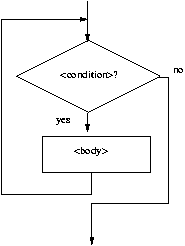
\includegraphics[width=4cm]{pic19}
  \end{center}
  \begin{itemize}
    \item uslov se ispituje \myblue{na vrhu} petlje
    \item ,,petlja sa izlaskom na vrhu``
    \item telo se može izvršiti 0 puta, 1 put, ili više puta
  \end{itemize}
}

\begin{frame}[fragile]
  \frametitle{Primeri \texttt{while} petlje}
\begin{itemize}
  \item primer \texttt{while} petlje koja broji od 0 do 10:
\end{itemize}
\begin{minted}{python}
i = 0
while i <= 10:
    print(i)
    i = i + 1
\end{minted}
\begin{itemize}
  \item isto radi kao i sledeća \texttt{for} petlja:
\end{itemize}
\begin{minted}{python}
for i in range(11):
    print(i)
\end{minted}
\end{frame}

\frame{
  \frametitle{\texttt{while} vs \texttt{for}}
  \begin{itemize}
    \item kod \texttt{while} petlje moramo sami da održavamo indeks petlje (\texttt{i})
    \item \myblue{inicijalizujemo} ga na 0 i ,,ručno`` ga \myblue{inkrementiramo} na kraju tela petlje
    \item kod \texttt{for} petlje ovo se odvija automatski
  \end{itemize}
}

\begin{frame}[fragile]
  \frametitle{\texttt{while} petlja: oprez}
  \begin{itemize}
    \item \texttt{while} petlja je moćnija
    \item predstavlja izvor mogućih grešaka
    \item kako radi ovaj kod?
  \end{itemize}
\begin{verbatim}
i = 0
while i <= 10:
    print(i)
\end{verbatim}
  \begin{itemize}
    \item<2> ovo je primer \myblue{beskonačne petlje}
  \end{itemize}
\end{frame}

\frame{
  \frametitle{Beskonačna petlja}
  \begin{itemize}
    \item šta da radimo ako program uđe u beskonačnu petlju?
    \item pritisnemo Ctrl-C
    \item ako ne pomogne, pritisnemo Ctrl-Alt-Del
    \item ako ne pomogne, resetujemo računar :)
  \end{itemize}
}

\section{Interaktivna petlja}

\frame{
  \frametitle{Interaktivna petlja}
  \begin{itemize}
    \item beskonačnu petlju možemo koristiti za pisanje \myblue{interaktivnih} petlji
    \item interaktivna petlja omogućava korisniku da ponavlja određeni deo programa neposredno na zahtev
    \item treba nam i način da evidentiramo koliko brojeva je uneto
    \item koristićemo još jedan akumulator -- \texttt{count}
  \end{itemize}
}

\begin{frame}[fragile]
  \frametitle{Interaktivna petlja $_2$}
  \begin{itemize}
    \item u svakom ciklusu petlje, pitaj korisnika da li ima još brojeva za unos
    \item taj odgovor pre početka mora biti ,,da`` da bismo ušli u prvi ciklus petlje
  \end{itemize}
\begin{verbatim}
postavi moredata na "yes"
while moredata == "yes"
   učitaj sledeći podatak
   obradi podatak
   pitaj korisnika da li ima još podataka
\end{verbatim}
\end{frame}

\begin{frame}[fragile]
  \frametitle{Interaktivna petlja $_3$}
  \begin{itemize}
    \item kombinujemo interaktivnu petlju i akumulatore za \texttt{sum} i \texttt{count}
  \end{itemize}
\begin{verbatim}
inicijalizuj sum na 0.0
inicijalizuj count na 0
postavi moredata na “yes”
while moredata == “yes”
   unesi broj x
   dodaj x na sum
   dodaj 1 na count
   pitaj korisnika da li ima još podataka
ispiši sum/count
\end{verbatim}
\end{frame}

\begin{frame}[fragile]
  \frametitle{Interaktivna petlja $_4$}
\begin{minted}{python}
# average2.py

def main():
    moredata = "da"
    sum = 0.0
    count = 0
    while moredata == 'da':
        x = eval(input("Unesite broj >> "))
        sum = sum + x
        count = count + 1
        moredata = input(
            "Ima još brojeva (da ili ne)? ")
    print("\nProsek je", sum / count)
\end{minted}
\end{frame}

\begin{frame}[fragile]
  \frametitle{Interaktivna petlja $_5$}
\begin{verbatim}
Unesite broj >> 32
Ima još brojeva (da ili ne)? da
Unesite broj >> 45
Ima još brojeva (da ili ne)? da
Unesite broj >> 34
Ima još brojeva (da ili ne)? da
Unesite broj >> 76
Ima još brojeva (da ili ne)? da
Unesite broj >> 45
Ima još brojeva (da ili ne)? jok

Prosek je 46.4
\end{verbatim}
\end{frame}

\section[Sentinel]{Sentinel petlja}

\begin{frame}[fragile]
  \frametitle{Sentinel petlja}
  \begin{itemize}
    \item \myblue{sentinel petlja} obrađuje podatke sve dok ne naiđe na specijalnu vrednost koja označava kraj
    \item ta specijalna vrednost zove se \myblue{sentinel}
    \item sentinel se mora razlikovati od ,,običnih`` podataka jer se on ne obrađuje
  \end{itemize}
\end{frame}

\begin{frame}[fragile]
  \frametitle{Sentinel petlja $_2$}
\begin{verbatim}
uzmi prvi podatak
while podatak nije sentinel
   obradi podatak
   uzmi naredni podatak
\end{verbatim}
  \begin{itemize}
    \item prvi podatak se izdvoji pre nego što petlja počne -- ,,priming read``
    \item ako je prvi podatak baš sentinel, petlja se preskače i nema obrade
    \item u suprotnom, podatak se obrađuje i čita se sledeći podatak
  \end{itemize}
\end{frame}

\begin{frame}[fragile]
  \frametitle{Sentinel petlja $_3$}
  \begin{itemize}
    \item recimo da računamo prosek pozitivnih brojeva
    \item neće biti broja manjeg od 0 -- negativan broj će biti sentinel
  \end{itemize}
\end{frame}

\begin{frame}[fragile]
  \frametitle{Sentinel i računanje proseka}
\begin{minted}{python}
# average3.py

def main():
    sum = 0.0
    count = 0
    x = eval(input(
        "Unesite broj (negativan za kraj) >> "))
    while x >= 0:
        sum = sum + x
        count = count + 1
        x = eval(input(
            "Unesite broj (negativan za kraj) >> "))
    print("\nProsek je", sum / count)
\end{minted}
\end{frame}

\begin{frame}[fragile]
  \frametitle{Sentinel i računanje proseka $_2$}
\begin{verbatim}
Unesite broj (negativan za kraj) >> 32
Unesite broj (negativan za kraj) >> 45
Unesite broj (negativan za kraj) >> 34
Unesite broj (negativan za kraj) >> 76
Unesite broj (negativan za kraj) >> 45
Unesite broj (negativan za kraj) >> -1

Prosek je 46.4
\end{verbatim}
\end{frame}

\begin{frame}[fragile]
  \frametitle{Sentinel i računanje proseka $_3$}
  \begin{itemize}
    \item ova verzija programa je jednostavna za korišćenje kao i prethodna (sa interaktivnom petljom)
    \item ali ne gnjavi korisnika sa unošenjem ,,da`` svaki put
    \item mana je što ne možemo raditi sa negativnim brojevima
    \item tada sentinel ne bi mogao biti broj
  \end{itemize}
\end{frame}

\begin{frame}[fragile]
  \frametitle{Sentinel i računanje proseka $_4$}
  \begin{itemize}
    \item mogli bismo unositi sve podatke kao stringove
    \item ispravan unos mora se konvertovati u broj
    \item sentinel bi mogao da bude prazan string -- \texttt{""}
  \end{itemize}
\end{frame}

\begin{frame}[fragile]
  \frametitle{Prazan string kao sentinel}
\begin{verbatim}
inicijalizuj sum na 0.0
inicijalizuj count na 0
unesi podatak kao string, xStr
while xStr != ""
   konvertuj xStr u broj x
   dodaj x na sum
   dodaj 1 na count
   unesi sledeći podatak kao string, xStr
ispiši sum / count
\end{verbatim}
\end{frame}

\begin{frame}[fragile]
  \frametitle{Prazan string kao sentinel $_2$}
\begin{minted}{python}
# average4.py

def main():
    sum = 0.0
    count = 0
    xStr = input(
        "Unesite broj (<Enter> za kraj) >> ")
    while xStr != "":
        x = eval(xStr)
        sum = sum + x
        count = count + 1
        xStr = input(
            "Unesite broj (<Enter> za kraj) >> ")
    print("\nProsek je", sum / count)
\end{minted}
\end{frame}

\begin{frame}[fragile]
  \frametitle{Prazan string kao sentinel $_3$}
\begin{verbatim}
Unesite broj (<Enter> za kraj) >> 34
Unesite broj (<Enter> za kraj) >> 23
Unesite broj (<Enter> za kraj) >> 0
Unesite broj (<Enter> za kraj) >> -25
Unesite broj (<Enter> za kraj) >> -34.4
Unesite broj (<Enter> za kraj) >> 22.7
Unesite broj (<Enter> za kraj) >>

Prosek je 3.38333333333
\end{verbatim}
\end{frame}

\section[Fajlovi]{Petlje i fajlovi}

\begin{frame}[fragile]
  \frametitle{Petlje i fajlovi}
  \begin{itemize}
    \item naš program je interaktivan -- to može biti nezgodno
    \item šta ako je korisnik pogrešio kod unosa 43. broja od njih 50?
    \item kod veće količine podataka bolje je čitati podatke iz fajla
  \end{itemize}
\end{frame}

\begin{frame}[fragile]
  \frametitle{Čitanje iz fajla u petlji}
\begin{minted}{python}
# average5.py

def main():
    fileName = input("Unesite ime fajla >> ")
    infile = open(fileName,'r')
    sum = 0.0
    count = 0
    for line in infile.readlines():
        sum = sum + eval(line)
        count = count + 1
    print("\nProsek je", sum / count)
\end{minted}
\end{frame}

\begin{frame}[fragile]
  \frametitle{Fajlovi i sentinel}
  \begin{itemize}
    \item mnogi jezici nemaju mogućnost za čitanje iz fajla pomoću \texttt{for} petlje
    \item tada je potreban sentinel
    \item možemo da koristimo \texttt{readline} u petlji da čitamo red-po-red iz fajla
    \item na kraju fajla \texttt{readline} će vratiti prazan string ""
    \begin{itemize}
      \item šta ako u fajlu postoji prazan red?
    \end{itemize}
  \end{itemize}
\end{frame}

\begin{frame}[fragile]
  \frametitle{Fajlovi i sentinel $_2$}
\begin{minted}{python}
line = infile.readline()
while line != ""
    # obradi line
    line = infile.readline()
\end{minted}
  \begin{itemize}
    \item da li ovaj kod pravilno radi u slučaju kada postoji prazan red u fajlu?
    \item za prazan red readline vraća \texttt{"\textbackslash n"}
  \end{itemize}
\end{frame}

\begin{frame}[fragile]
  \frametitle{Fajlovi i sentinel $_2$}
\begin{minted}{python}
# average6.py

def main():
    fileName = input("Unesite ime fajla >> ")
    infile = open(fileName,'r')
    sum = 0.0
    count = 0
    line = infile.readline()
    while line != "":
        sum = sum + eval(line)
        count = count + 1
        line = infile.readline()
    print("\nProsek je", sum / count)
\end{minted}
\end{frame}

\section[Ugnježdavanje]{Ugnježdene petlje}

\begin{frame}[fragile]
  \frametitle{Ugnježdene petlje}
  \begin{itemize}
    \item videli smo kako je moguće ugnježdavati \texttt{if} naredbe
    \item na sličan način je moguće ugnježdavati i petlje
    \item recimo da u fajlu sa brojevima, u jednom redu može biti više brojeva razdvojenih zarezom
  \end{itemize}
\end{frame}

\begin{frame}[fragile]
  \frametitle{Ugnježdene petlje $_2$}
  \begin{itemize}
    \item na najvišem nivou koristićemo petlju za obradu fajla koja računa \texttt{sum} i \texttt{count}
  \end{itemize}
\begin{minted}{python}
sum = 0.0
count = 0
line = infile.readline()
while line != "":
    # ažuriraj sum i count
    line = infile.readline()
print("\nProsek je", sum/count)
\end{minted}
\end{frame}

\begin{frame}[fragile]
  \frametitle{Ugnježdene petlje $_3$}
  \begin{itemize}
    \item na sledećem nivou treba ažurirati \texttt{sum} i \texttt{count}
    \item pošto svaki red u fajlu sadrži više brojeva razdvojenih zarezom, možemo taj string podeliti na podstringove
    \item svaki od podstringova će biti broj
    \item u petlji idemo kroz sve podstringove, \\
    \ \ \ \ konvertujemo ih u broj \\
    \ \ \ \ i dodajemo na \texttt{sum} \\
    \ \ \ \ i inkrementiramo \texttt{count}
  \end{itemize}
\end{frame}

\begin{frame}[fragile]
  \frametitle{Ugnježdene petlje $_4$}
\begin{minted}{python}
for xStr in line.split(","):
    sum = sum + eval(xStr)
    count = count + 1
\end{minted}
  \begin{itemize}
    \item ova \texttt{for} petlja koristi \texttt{line}, što je promenljiva iz spoljne petlje
  \end{itemize}
\end{frame}

\begin{frame}[fragile,shrink=5]
  \frametitle{Ugnježdene petlje $_5$}
\begin{minted}{python}
# average7.py

import string

def main():
    fileName = input("Unesite ime fajla >> ")
    infile = open(fileName, 'r')
    sum = 0.0
    count = 0
    line = infile.readline()
    while line != "":
        for xStr in line.split(","):
            sum = sum + eval(xStr)
            count = count + 1
        line = infile.readline()
    print("\nProsek je", sum / count)

\end{minted}
\end{frame}

\begin{frame}[fragile]
  \frametitle{Ugnježdene petlje $_6$}
  \begin{itemize}
    \item petlja koja obrađuje brojeve u jednom redu je uvučena ispod petlje koja čita redove iz fajla
    \item spoljašnja while petlja iterira jednom za svaki red u fajlu
    \item za svaki ciklus spoljašnje petlje, unutrašnja petlja iterira sve cikluse (zavisno od broja brojeva u tom redu)
    \item kada se završi unutrašnja petlja, čita se sledeći red i proces se ponavlja
  \end{itemize}
\end{frame}

\section{Bulova algebra}

\begin{frame}[fragile]
  \frametitle{Logički izrazi}
  \begin{itemize}
    \item \texttt{if} i \texttt{while} koriste logičke (Bulove) izraze
    \item vrednost logičkog izraza može biti \texttt{True} ili \texttt{False}
    \item do sada smo pisali samo izraze poređenja (\texttt{while x>0:})
  \end{itemize}
\end{frame}

\begin{frame}[fragile]
  \frametitle{Logički operatori}
  \begin{itemize}
    \item ovakvi jednostavni izrazi nekad nisu dovoljni
    \item recimo da treba odrediti da su dve 2D tačke na istom mestu
    \item njihove $x$ koordinate moraju biti jednake
    \item i $y$ koordinate moraju biti jednake
  \end{itemize}
\end{frame}

\begin{frame}[fragile]
  \frametitle{Logički operatori $_2$}
\begin{minted}{python}
if x1 == x2:
    if y1 == y2:
        # tačke su jednake
    else:
        # tačke nisu jednake
else:
    # tačke nisu jednake
\end{minted}
  \begin{itemize}
    \item ovakav test izgleda rogobatno
    \item možemo koristiti logičke operatore \texttt{and}, \texttt{or} i \texttt{not}
  \end{itemize}
\end{frame}

\begin{frame}[fragile]
  \frametitle{Operatori \texttt{and} i \texttt{or}}
  \begin{itemize}
    \item operatori \texttt{and} i \texttt{or} se koriste za kombinovanje \myblue{dva} logička izraza i daju logički rezultat
    \item očekuju dva \myblue{operanda}: zovemo ih \myblue{binarni} operatori
  \end{itemize}
\begin{verbatim}
<izraz1> and <izraz2>
<izraz1> or <izraz2>
\end{verbatim}
\end{frame}

\begin{frame}[fragile]
  \frametitle{Operator \texttt{and}}
  \begin{itemize}
    \item operator \texttt{and} predstavlja konjunkciju dva logička izraza
    \item vraća \texttt{True} samo kad su \myblue{oba} izraza \texttt{True}
  \end{itemize}
  \begin{center}
  \begin{tabular}{c|c|c}
    \texttt{P} & \texttt{Q} & \texttt{P and Q} \\ \hline
    T & T & T \\ \hline
    T & F & F \\ \hline
    F & T & F \\ \hline
    F & F & F
  \end{tabular}
  \end{center}
  \begin{itemize}
    \item \texttt{P} i \texttt{Q} su operandi
    \item postoji 4 moguće kombinacije vrednosti
  \end{itemize}
\end{frame}

\begin{frame}[fragile]
  \frametitle{Operator \texttt{or}}
  \begin{itemize}
    \item operator \texttt{or} predstavlja disjunkciju dva logička izraza
    \item vraća \texttt{True} ako je \myblue{bilo koji} od izraza \texttt{True}
  \end{itemize}
  \begin{center}
  \begin{tabular}{c|c|c}
    \texttt{P} & \texttt{Q} & \texttt{P or Q} \\ \hline
    T & T & T \\ \hline
    T & F & T \\ \hline
    F & T & T \\ \hline
    F & F & F
  \end{tabular}
  \end{center}
  \begin{itemize}
    \item \texttt{or} vraća \texttt{False} samo kad su oba operanda \texttt{False}
    \item \texttt{or} vraća \texttt{True} kad su oba operanda \texttt{True} -- to se razlikuje od korišćenja reči ,,ili`` u prirodnom jeziku!
  \end{itemize}
\end{frame}

\begin{frame}[fragile]
  \frametitle{Operator \texttt{not}}
  \begin{itemize}
    \item operator \texttt{not} predstavlja negaciju logičkog izraza
    \item not je \myblue{unarni} operator -- ima jedan operand
  \end{itemize}
  \begin{center}
  \begin{tabular}{c|c}
    \texttt{P} & \texttt{not P} \\ \hline
    T & F \\ \hline
    F & T 
  \end{tabular}
  \end{center}
\end{frame}

\begin{frame}[fragile]
  \frametitle{Kombinovanje logičkih operatora}
  \begin{itemize}
    \item operatore možemo kombinovati i tako graditi složene izraze
    \item izračunavanje takvih izraza zavisi od \myblue{prioriteta operatora}
    \item prioritet operatora je u opadajućem redosledu: \texttt{not}, \texttt{and}, \texttt{or}
    \item na primer: \\ \texttt{a or not b and c}
    \item je isto što i \\ \texttt{(a or ((not b) and c))}
    \item treba koristiti zagrade da se izbegne zabuna
  \end{itemize}
\end{frame}

\begin{frame}[fragile]
  \frametitle{Kombinovanje logičkih operatora $_2$}
  \begin{itemize}
    \item za poređenje 2D tačaka možemo koristiti \texttt{and}
  \end{itemize}
\begin{minted}{python}
if x1 == x2 and y1 == y2:
    # tačke su jednake
else:
    # tačke nisu jednake
\end{minted}
  \begin{itemize}
    \item ceo izraz će biti \texttt{True} samo kada su \myblue{oba} manja izraza \texttt{True}
  \end{itemize}
\end{frame}

\begin{frame}[fragile]
  \frametitle{Racquetball}
  \begin{itemize}
    \item sport sa reketom i lopticom u zatvorenom prostoru, slično skvošu
    \item igra se dok jedan od igrača ne osvoji 15 poena \\
      \texttt{scoreA == 15 or scoreB == 15}
    \item kada je bar jedan od izraza \texttt{True}, ceo izraz je \texttt{True}
    \item treba nam petlja koja radi sve dok igra \myblue{nije završena}
    \item možemo negirati gornji izraz:
  \end{itemize}
\begin{verbatim}
while not(scoreA == 15 or scoreB == 15):
    # nastavi da igraš
\end{verbatim}
\end{frame}

\begin{frame}[fragile]
  \frametitle{Racquetball $_2$}
  \begin{itemize}
    \item ako jedan igrač osvoji 7 poena dok drugi ne osvoji nijedan, igra se završava
  \end{itemize}
\begin{minted}{python}
while not(scoreA == 15 or scoreB == 15 or 
  (scoreA == 7 and scoreB == 0) or 
  (scoreB == 7 and scoreA == 0):
    # nastavi da igraš
\end{minted}
\end{frame}

\begin{frame}[fragile]
  \frametitle{Odbojka}
  \begin{itemize}
    \item jedan set se igra do 25 poena
    \item set se mora dobiti sa 2 poena razlike
  \end{itemize}
\begin{minted}{python}
(a >= 25 and a-b >= 2) or (b >= 25 and b-a >= 2)

(a >= 25 or b >= 25) and abs(a-b) >= 2
\end{minted}
\end{frame}

\begin{frame}[fragile]
  \frametitle{Bulova algebra}
  \begin{itemize}
    \item veština pisanja logičkih izraza je veoma važna
    \item logički izrazi poštuju zakone \myblue{Bulove algebre}
  \end{itemize}
  \begin{center}
  \begin{tabular}{l|l}
    \textbf{algebra} & \textbf{Bulova algebra} \\ \hline
    $a\cdot 0 = 0$ & \texttt{a and False == False} \\ \hline
    $a\cdot 1 = a$ & \texttt{a and True == a} \\ \hline
    $a + 0 = a$ & \texttt{a or False == a}
  \end{tabular}
  \end{center}
  \begin{itemize}
    \item \texttt{and} liči na množenje
    \item \texttt{or} liči na sabiranje
    \item 0 liči na \texttt{False}, 1 liči na \texttt{True}
  \end{itemize}
\end{frame}

\begin{frame}[fragile]
  \frametitle{Bulova algebra $_2$}
  \begin{itemize}
    \item bilo šta \texttt{or}-ovano sa \texttt{True} je \texttt{True} \\
      \texttt{a or True == True}
    \item distributivnost \texttt{and} i \texttt{or} \\
      \texttt{a or (b and c) == (a or b) and (a or c)} \\
      \texttt{a and (b or c) == (a and b) or (a and c)}
    \item dvostruka negacija se poništava \\
      \texttt{not(not a) == a}
    \item De Morganovi zakoni \\
      \texttt{not(a or b) == (not a) and (not b)} \\
      \texttt{not(a and b) == (not a) or (not b)}
  \end{itemize}
\end{frame}

\begin{frame}[fragile]
  \frametitle{Bulova algebra $_3$}
  \begin{itemize}
    \item na osnovu ovih pravila možemo pojednostaviti neke izraze
  \end{itemize}
\begin{minted}{python}
while not(scoreA == 15 or scoreB == 15):
    # nastavi da igraš
\end{minted}
  \begin{itemize}
    \item primenom De Morganovog zakona
  \end{itemize}
\begin{minted}{python}
while (not scoreA == 15) and (not scoreB == 15):
    # nastavi da igraš
\end{minted}
  \begin{itemize}
    \item što se svodi na
  \end{itemize}
\begin{minted}{python}
while scoreA != 15 and scoreB != 15:
    # nastavi da igraš
\end{minted}
\end{frame}

\begin{frame}[fragile]
  \frametitle{Bulova algebra $_4$}
  \begin{itemize}
    \item nekad je lakše formulisati uslov kada petlja treba da se završi, nego kada da nastavi sa radom
    \item samo dodamo \texttt{not} na početak takvog izraza
    \item pomoću De Morganovih zakona možemo dalje pojednostaviti izraz
  \end{itemize}
\end{frame}

\section[Petlje 2]{Još o petljama}

\begin{frame}[fragile]
  \frametitle{Petlja sa izlaskom na dnu}
  \begin{itemize}
    \item \texttt{for} i \texttt{while} mogu da posluže da izrazimo bilo koji algoritam
    \item međutim, nekada je čitljivije koristiti petlje sa izlaskom na dnu (umesto na vrhu)
    \item primer:
  \end{itemize}
\begin{verbatim}
repeat
    unesi broj 
until number >= 0
\end{verbatim}
\end{frame}

\begin{frame}[fragile]
  \frametitle{Petlja sa izlaskom na dnu $_2$}
  \begin{center}
    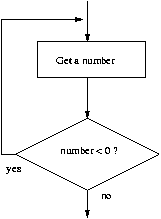
\includegraphics[width=5cm]{pic20}
  \end{center}
\end{frame}

\begin{frame}[fragile]
  \frametitle{Petlja sa izlaskom na dnu $_3$}
  \begin{itemize}
    \item telo petlje sa izlaskom na dnu izvrši se \myblue{obavezno} bar jednom
    \item Python nema naredbu za ovakve petlje ali se ona može napraviti pomoću \texttt{while}
    \item pripremimo vrednosti tako da uslov bude uvek ispunjen pre prvog ciklusa petlje
  \end{itemize}
\begin{minted}{python}
number = -1
while number < 0:
    # uradi nešto
\end{minted}
\end{frame}

\begin{frame}[fragile]
  \frametitle{Petlja sa izlaskom na dnu $_4$}
  \begin{itemize}
    \item u Pythonu se ovakva petlja može simulirati i pomoću \texttt{break} naredbe
    \item \texttt{break} služi za momentalno iskakanje iz petlje
    \item može i za iskakanje iz beskonačne petlje
  \end{itemize}
\begin{minted}{python}
while True:
    number = eval(input("Unesite broj >> "))
    if number >= 0: 
        break # izađi iz petlje ako je broj ispravan
\end{minted}
  \begin{itemize}
    \item bilo bi lepo da program ispiše upozorenje da broj nije ispravan
  \end{itemize}
\end{frame}

\begin{frame}[fragile]
  \frametitle{Petlja sa izlaskom na dnu $_5$}
  \begin{itemize}
    \item u verziji sa \texttt{while} petljom ovo je rogobatno
  \end{itemize}
\begin{minted}{python}
number = -1
while number < 0:
    number = eval(input("Unesite pozitivan broj: "))
    if number < 0:
        print("Uneti broj nije pozitivan!")
\end{minted}
  \begin{itemize}
    \item vršimo proveru na dva mesta -- nije elegantno
  \end{itemize}
\end{frame}

\begin{frame}[fragile]
  \frametitle{Petlja sa izlaskom na dnu $_6$}
  \begin{itemize}
    \item verzija sa \texttt{break} samo još dodaje \texttt{else} klauzulu
  \end{itemize}
\begin{minted}{python}
while True:
    number = eval(input("Unesite pozitivan broj: "))
    if number >= 0:
        break
    else:
        print("Uneti broj nije pozitivan!")
\end{minted}
\end{frame}

\begin{frame}[fragile]
  \frametitle{Petlja ipo}
  \begin{itemize}
    \item nešto elegantnija verzija
  \end{itemize}
\begin{minted}{python}
while True:
    number = eval(input("Unesite pozitivan broj: "))
    if number >= 0: 
        break
    print("Uneti broj nije pozitivan!")
\end{minted}
  \begin{itemize}
    \item izlaz iz petlje je u sredini tela petlje
    \item $\rightarrow$ ,,\myblue{petlja ipo}``
  \end{itemize}
\end{frame}

\begin{frame}[fragile]
  \frametitle{Petlja ipo}
  \begin{itemize}
    \item petlja ipo je elegantan način da se izbegne inicijalno čitanje u sentinel petlji
  \end{itemize}
\begin{verbatim}
while True:
    uzmi sledeći podatak
    if podatak je sentinel: 
        break
    obradi podatak
\end{verbatim}
  \begin{itemize}
    \item sentinel vrednost se ne obrađuje
    \item ne moramo inicijalizovati ništa pre petlje
  \end{itemize}
\end{frame}

\begin{frame}[fragile]
  \frametitle{Petlja ipo}
  \begin{center}
    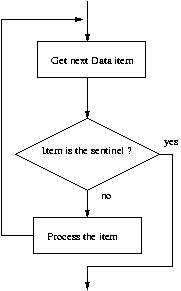
\includegraphics[width=4cm]{pic21}
  \end{center}
\end{frame}

\begin{frame}[fragile]
  \frametitle{Koristiti \texttt{break}: da ili ne?}
  \begin{itemize}
    \item korišćenje \texttt{break} je stvar ukusa
    \item zbog lakšeg čitanja koda, \texttt{break} treba koristiti samo kad je neophodno
    \item teško je pratiti kod u kome ima više \texttt{break}-ova za izlazak iz petlje
  \end{itemize}
\end{frame}

\section[Logički izrazi]{Logički izrazi i grananje}

\begin{frame}[fragile]
  \frametitle{Logički izrazi i grananje}
  \begin{itemize}
    \item logički izrazi se mogu koristiti za kontrolu toka programa
    \item recimo da pišemo program koji se izvršava sve dok korisnik unosi odgovor koji počinje sa \texttt{"y"}
    \item jedno rešenje: \\
      \texttt{while response[0] == "y" or response[0] == "Y":}
  \end{itemize}
\end{frame}

\begin{frame}[fragile]
  \frametitle{Logički izrazi i grananje $_2$}
  \begin{itemize}
    \item samo pažljivo! ne možemo pisati ,,skraćeno``: \\
      \texttt{while response[0] == "y" or "Y":}
    \item zašto ovo ne radi?
    \item Python interno predstavlja \texttt{bool} tip pomoću brojeva \\ 1 (za \texttt{True}) i 0 (za \texttt{False})
    \item relacioni operatori kao \texttt{==} uvek vraćaju \texttt{bool} vrednost
  \end{itemize}
\end{frame}

\begin{frame}[fragile,shrink=10]
  \frametitle{Logički izrazi i grananje $_3$}
  \begin{itemize}
    \item Python će dopustiti da se svaki drugi tip tretira kao \texttt{bool}
    \item za brojeve: 0 se smatra za \texttt{False}, sve ostalo je \texttt{True}
    \item za liste: prazna lista je \texttt{False}, neprazna je \texttt{True}
    \item za stringove: prazan string je \texttt{False}, neprazan je \texttt{True}
  \end{itemize}
\begin{minted}{python}
>>> bool(0)
False
>>> bool(1)
True
>>> bool(32)
True
>>> bool("Hello")
True
>>> bool("")
False
>>> bool([1,2,3])
True
>>> bool([])
False
\end{minted}
\end{frame}

\begin{frame}[fragile]
  \frametitle{Logički operatori i drugi tipovi podataka}
  \begin{itemize}
    \item logičke operatore možemo primeniti i na druge tipove podataka, ne samo \texttt{bool}
    \item značenje operatora u tom slučaju je sledeće:
  \end{itemize}
  \begin{center}
    \begin{tabular}{l|l}
      \textbf{operator} & \textbf{značenje} \\ \hline
      \texttt{x and y} & ako je \texttt{x} \texttt{False} vrati \texttt{x}, inače vrati \texttt{y} \\ \hline
      \texttt{x or y} & ako je \texttt{x} \texttt{True} vrati \texttt{x}, inače vrati \texttt{y} \\ \hline
      \texttt{not x} & ako je \texttt{x} \texttt{False} vrati \texttt{True}, inače vrati \texttt{False}
    \end{tabular}
  \end{center}
\end{frame}

\begin{frame}[fragile]
  \frametitle{Operator \texttt{and} i drugi tipovi podataka}
  \begin{itemize}
    \item razmotrimo izraz \texttt{x and y}
    \item ako je \texttt{x} \texttt{True}, tada vrednost celog izraza zavisi od \texttt{y}
    \item vraćanjem \texttt{y}, ako je \texttt{y} \texttt{True}, \texttt{True} se i vraća
    \item ako je \texttt{y} \texttt{False}, \texttt{False} se i vraća
  \end{itemize}
\end{frame}

\begin{frame}[fragile]
  \frametitle{Izračunavanje logičkih izraza}
  \begin{itemize}
    \item prilikom izračunavanja logičkog izraza True ili False se vraćaju čim je rezultat poznat
    \item ne mora se ceo izraz izračunati!
    \item u \texttt{and}-izrazu, ako je prvi operand \texttt{False}, rezultat je obavezno \texttt{False}
    \item u \texttt{or}-izrazu, ako je prvi operand \texttt{True}, rezultat je obavezno \texttt{True}
  \end{itemize}
\end{frame}

\begin{frame}[fragile]
  \frametitle{Izračunavanje logičkih izraza: primer}
  \begin{itemize}
    \item pogledajmo izraz \\
      \texttt{response[0] == "y" or "Y"}
    \item on je isto što i \\
      \texttt{(response[0] == "y") or ("Y")}
    \item da bi ovaj izraz bio \texttt{True}:
    \begin{itemize}
      \item treba da je \texttt{response[0] == "y"}
      \item \texttt{"Y"} je neprazan string -- tretira se kao \texttt{True}
    \end{itemize}
    \item ovaj izraz će uvek biti \texttt{True}, bez obzira šta korisnik unese!
  \end{itemize}
\end{frame}

\begin{frame}[fragile]
  \frametitle{Izračunavanje logičkih izraza: primer 2}
\begin{minted}{python}
ans = input("Koji sladoled želite [vanila]: ")
if ans:
    flavor = ans
else:
    flavor = "vanila"
\end{minted}
  \begin{itemize}
    \item ako korisnik samo pritisne Enter, \texttt{ans} će biti prazan string
    \item prazan string se tretira kao \texttt{False}
  \end{itemize}
\end{frame}

\begin{frame}[fragile,shrink=5]
  \frametitle{Izračunavanje logičkih izraza: primer 2 $_2$}
  \begin{itemize}
    \item ovo može još sažetije!
  \end{itemize}
\begin{minted}{python}
ans = input("Koji sladoled želite [vanila]: ")
flavor = ans or "vanila"
\end{minted}
  \begin{itemize}
    \item ili još kraće:
  \end{itemize}
\begin{minted}{python}
flavor = input("Koji sladoled [vanila]: ") or "vanila"
\end{minted}
\end{frame}

\begin{frame}[fragile]
  \frametitle{Izračunavanje logičkih izraza}
  \begin{itemize}
    \item ovakav kod može biti teško razumljiv
    \item zbog čitljivosti -- treba se uzdržati od prekomerne upotrebe ovih ,,trikova``
  \end{itemize}
\end{frame}


\end{document}